% Requires Latex2e!
\documentclass[cyr]{bibl}

\firstpage{1}
\lastpage{12}
\titlepage{}

\usepackage{geometry}
\usepackage{ragged2e}
\usepackage{amssymb}

%%%%%% NA OVOM MESTU DEFINISETE LATEX KOMANDE
%%%%%% Na primer: \newcommand{\const}{\mathop{\mathrm{const}}}
\newgeometry{top = 12cm}

\begin{document}

\title{ Primena fazi logike u ocenjivanju filmova na bazi recenzija gledalaca}
\author{{\fnms{  Dunja{}} \snm{Spasi\cc{}}}}
\address{  Matematichki fakultet\\
\email{mi16073@alas.matf.bg.ac.rs}}
\author{{\fnms{  Jelena{}} \snm{ Jeremi\cc{}}}}
\address{  Matematichki fakultet\\
\email{mi16062@alas.matf.bg.ac.rs}}

\Large
\maketitle


\newpage
\newgeometry{top = 5cm}
\RaggedRight
\section{Problem predvidjanja ocene filma}
\begin{justify}

Na internetu postoji veliki broj sajtova za pretragu mnogih usluga ili proizvoda. Takvi sajtovi obichno dopushtaju korisnicima da daju komentar i ocenu sadrzhaja koji sajt nudi. Problem kojim se ovaj projekat bavi je dodela ocene filmu na osnovu unete recenzije gledaoca. Mogu\cc e je, sa nekim izmenama, primeniti ovaj program i na druge vrste usluga. Za potrebe ovog projekta je korish\cc en sajt \textit{\Lat IMDb} tako shto su za bazu komentara i ocena su uzete recenzije za 18 ljubavnih filmova. Cilj ovog projekta je da se korisniku predlozhi ocena koju bi mogao da da filmu na osnovu komentara koji je uneo. Ovaj problem mozhe da se posmatra kao problem klasifikacije.

U radu [1] je slichan problem reshavan primenom algoritama za klasifikaciju podataka. Autori su klasifikovali recenzije filmova u pet klasa, od najmanje do najvishe korisne u zavisnosti od zajednichkih interesovanja autora recenzije i korisnika. Primenjeni su algoritam Bajesove klasifikacije i neuronske mrezhe.

Rad [2] se bavi analizom polarnosti ose\cc anja u recenzijama filmova napisanih na shpanskom jeziku. Autori su pristupili ovom problemu tehnikama istrazhivanja mishljenja (eng. \textit{\Lat Opinion Mining}) i semantichkog orijentisanja (eng. \textit{\Lat Semantic Orientation}). Istrazhivanje mishljenja podrazumeva sakupljanje stvarnih podataka i analizu novih podataka na osnovu napravljene baze pa spada u metode nadgledanog uchenja. Semantichko orijentisanje je metoda koja ne analizira podatke uchenjem. Ovaj pristup ukljuchuje pam\cc enje pozitivnih i negativnih rechi, a zatim odredjuje da li se rechi iz recenzije nalaze u prvom ili drugom skupu. Obe metode imaju i prednosti i mane. Mana istrazhivanja mishljenja je shto se skup rechi previshe oslanja na sakupljenje podatke. S druge strane, mana semantichkog orijentisanja je potreba za chuvanjem velikih rechnika, a i nedovoljna fleksibilnost algoritma pri promeni korish\cc enog jezika. Kao i u radu [2], ovaj projekat kombinuje obe metode.  
\end{justify}

\pagebreak

\section{Reshenje problema korish\cc enjem fazi logike}
\begin{justify}

Prilikom reshavanja ovog zadatka bilo je potrebno formalnim, matematichkim jezikom opisati prirodan jezik, tj. uchiniti da program razume recenziju napisanu na prirodnom jeziku. Za reshavanje problema izabrane su metode fazi logike. Na osnovu unete recenzije, odredjuje se vrednost iz realnog intervala [0,1] koja predstavlja stepen pripadnosti filma skupu dobrih filmova. Prednost upotrebe fazi logike i funkcije pripadnosti skupu dobrih filmova je elegantno reshenje situacije da se recenzijom uglavnom iznose i dobre i loshe karakteristike filma, shto podrazumeva da ve\cc ina filmova ne\cc e biti ni potpuno dobri ni potpuno loshi. Druga prednost ovakvog nachina ocenjivanja je shto se interval [0,1] lako preslikava na ocene od 1 do 10.

Na samom pochetku \textit{\Lat IMDb User reviews} stranice su razdvojene tako shto su iz svake rechenice recenzije sachuvane bitne rechi, tj. izbacuju se tzv. \textit{\Lat stop words}, rechi koje se chesto pojavljuju u rechenicama ali ne igraju nikakvu ulogu u znachenju rechenice. Ove rechi su sadrzhane u \textit{\Lat python} biblioteci \textit{\Lat nltk.corpus}. Osim \textit{\Lat stop} rechi iz recenzija su izbacheni i modifikatori, chija \cc e uloga kasnije da bude objashnjena. Parovi \textit{\Lat (lista bitnih reci, ocena komentara)} su formirani na osnovu recenzija svih 18  korish\cc enih filmova i sachuvani u \textit{\Lat csv} fajlu. Zatim su napravljenje dve mape, od kojih jedna sadrzhi sve bitne rechi koje se pojavljuju u recenzijama filmova ocenjenih sa 1, 2 i 3, dok druga mapa sadrzhi rechi koje se pojavljuju u recenzijama filmova ocenjenih sa 8, 9 i 10. Kljuchevi elemenata mapa su rechi, a vrednosti su broj pojavljivanja u loshim recenzijama i broj pojavljivanja u dobrim recenzijama. Ova dva skupa rechi su uslovno nazvana skupom dobrih rechi i skupom loshih rechi u zavisnosti od toga da li hvale film ili ga kritikuju. Za odluchivanje da li rech pripada skupu dobrih ili loshih rechi je bilo presudno u kojim recenzijama se frekventnije pojavljuje. Intuitivno bi bilo uzimati razliku te dve frekventnosti kao vrednost u mapi, jer ako se rech pojavljuje isti broj puta i u pozitivnim i u negativnim komentarima, ona mozhe da deluje neutralno. Medjutim, na osnovu recenzija je prime\cc eno da su se pozitivne rechi u velikom broju javljale u negativnim recenzijama u formi negacije. Frekventnost pojavljivanja dobre rechi u loshim komentarima ne umanjuje njen znachaj kao dobre rechi, pa je za vrednost uzet maksimum ta dva pojavljivanja.

Fazi funkcije pripadnosti su definisane trapezoidnim funkcijama. Funkcija dobrih rechi (slika 1. levo) ima znachajne tachke (0,0) i (110,1), a funkija loshih rechi (slika 1. desno) ima znachajne tachke (0,1) i (60,0). Ovo znachi da kako se pove\cc ava broj pojavljivanja dobrih rechi u recenziji, tako raste vrednost funkcije pripadnosti skupu dobrih filmova, a kako raste broj pojavljivanja loshih rechi tako opada vrednost funkcije pripadnosti skupu dobrih filmova. 

\begin{figure}[ht!]
\centering
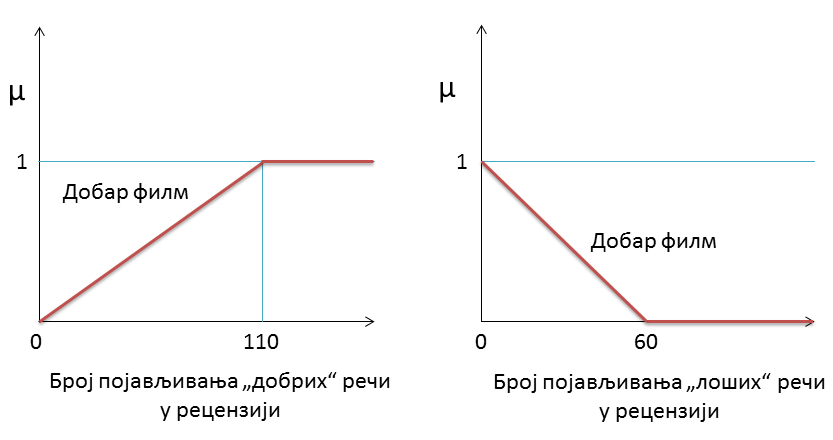
\includegraphics[width=1.0\textwidth]{fazi2.png}
\caption{Funkcije pripadnosti fazi skupu.}\label{sample image}
\end{figure}


Lingvistichke promenljive su promenljive chije su vrednosti rechi prirodnog jezika. Vrednost ovih promenljivih mozhe da se pove\cc a ili smanji primenom modifikatora. U prirodnim jezicima oni obichno predstavljaju neke prideve ili priloge. Postoje razlichite vrste modifikatora:
\begin{itemize}
    \begin{justify}
    \item \textbf{Koncentracioni}, koji jachaju vrednosti promenljivih uz koje stoje tj. utichu tako da vrednosti funkcije postanu vishe koncetrisane oko tachaka sa ve\cc im stepenom pripadnosti.
    
    \centering\(\mu_{A'}(x) = \mu_{A}(x)^{\frac{1}{p}}\)  za \textit{\Lat p} ve\cc e od 1
    \end{justify}
    \begin{justify}
	\item \textbf{Dilatacioni}, kojima se vrednost funkcije pripadnosti smanjuje.
	
    \centering\(\mu_{A'}(x) = \mu_{A}(x)^{p}\)  za \textit{\Lat p} ve\cc e od 1
    
    \end{justify}
	
\end{itemize} 
\newline
\newline
Pored ovih postoje josh i: kontrastni intenzifikatori, kontrastni deintenzifikatori, probabilistichki... U daljem radu koristi\cc emo prve dve vrste modifikatora.

U sluchaju problema recenzija filmova, lingvistichke promenljive su rechi koje se pojavljuju u recenzijama sa visokim ili niskim ocenama, tj. bitne rechi. Modifikatori ovde predstavljaju rechi koje chesto stoje uz bitne rechi i dodatno ih opisuju, pojachavaju\cc i ili umanjuju\cc i njihovo znachenje. Modifikatori su podeljeni u tri grupe, na osnovu toga koliko jachaju znachenje bitne rechi, a u zavisnosti od toga u koju od te tri grupe spadaju, dodeljene su im i ocene.

Modifikatori koji slabije utichu na znachenje bitne rechi su ocenjeni sa 2, oni koji osrednje utichu su ocenjeni sa 3, a oni koji izuzetno doprinose jachini bitnih rechi, su ocenjeni sa 4.
Modifikatori su izdvojeni u poseban \textit{\Lat Python} datoteku radi laksheg rada sa njima. Konachna ocena bitne rechi zavisila je od toga da li rech pripada skupu dobrih ili loshih rechi. Ukoliko rech pripada skupu dobrih rechi i modifikator uz tu rech jacha znachenje rechi, tada se ocena \(\mu\) te rechi racunala kao \(\mu^{\frac{1}{p}}\) gde je \textit{\Lat p} ocena jachine ovog modifikatora, a ukoliko modifikator slabi rech, ocena je rachunata kao \(\mu^{p}\). Obrnuto se rachunala ocena za rech koja pripada skupu loshih rechi. Ako bi se rech nashla u oba skupa, tada je posmatrano da li je ve\cc i broj rechi u toj rechenici iz skupa dobrih ili loshih rechi.

Obrada samih komentara odvojena je od fazi logike. Komentari su bivali prochish\cc eni od rechi koje nisu pripadale skupu bitnih rechi, ali su takodje morali da se chuvaju i celi komentari kako bi se vrshila provera da li se uz bitnu rech nalazi neki modifikator koji bi mogao promeniti vrednost ove lingvistichke promenljive ili rech \textit{\Lat not} koja u potpunosti menja znak vrednosti funkcije za tu lingvistichku promenljivu.
Zarad lakshe obrade, skup prochish\cc enih rechi i skup sa svakom rechju iz komentara su predstavljeni listama. Nakon razvrstavanja ovih rechi u odgovaraju\cc e liste, skupovi su bivali prosledjeni glavnom programu za konachnu obradu i dodelu ocene komentaru.
\end{justify}

\newpage
\section{Rezultati primene reshenja}
\begin{justify}
Reshenje je testirano na recenzijama sa ocenama iz intervala od 4 do 7, s obzirom da je program obuchavan na recenzijama sa najnizhim i najvishim ocenama (od 1 do 3 i od 8 do 9).

Naknadno je uocheno da rech \textit{\Lat not} ne mozhe da se posmatrata kao modifikator jer ona menja celokupno znachenje komentara, tj. \textit{\Lat not} predstavlja logichku negaciju, dobre bitne rechi pretvara u loshe, a loshe u dobre. Negacija je implementirana kao \(1 - \mu\), jer fazi funkcije imaju suprotne monotonosti, a zatim se novo \(\mu\) pomnozhi sa -1 kako bi se dodalo na konachni rezultat. Nakon ispravke ovog dela, ocene su pochele sve bolje da oslikavaju unete recenzije.

Prvo su bile testirane znachajne tachke (0,0) i (60,1) za fazi funkciju dobrih rechi i (0,1) i (60,0) za fazi funkciju loshih rechi. Poshto se dobre rechi chesh\cc e pojavljuju od loshih, veliki broj njih je imao fazi vrednost 1. Ovo je loshe kada se uzmu u obzir i modifikatori, jer pozitivni modifikatori na ovakve rechi ne bi imali nikakav uticaj. Zato je u fazi funkciji dobrih rechi druga tachka pomerena na (110,1). Nakon kasnijeg obradjivanja svih komentara i eksperimentalnih pomeranja krajnjih tachaka u fazi funkcijama, zakljucheno je da tachke (110,1) za funkciju dobrih rechi i (60,0) za funkciju loshih rechi daju najbolje rezultate.  

Problem defazifikacije je reshen na slede\cc i nachin: ocene filmova se kre\cc u u segmentu od [1, 10], a ukupna ocena \(\mu\) je rachunata kao zbir svih ocena bitnih rechi podeljen sa brojem bitnih rechi. Kako smo imali i pozitivne i negativne recenzije i na osnovu dodele ocena pozitivnim i negativnim recenzijama, ukupan \(\mu\) se kretao u intervalu od -1 do 1.
Ovaj interval je podeljen na 10 jednakih delova tako da ukoliko bi se ukupan \(\mu\) nashao u intervalu od -1 do 0, recenzija bi bila ocenjena sa nekom od ocena iz segmenta [1, 5]. Ukoliko bi se ukupan \(\mu\) nasao u pozitivnom delu intervala, tada bi se recenziji dodeljivale vishe ocene, iz segmenta [6, 10]. Korish\cc enje intervala [-1,1], tj. oduzimanja loshih rechi i sabiranja dobrih reshava problem pojavljivanja novih rechi koje se nikada nisu pojavile u recenzijama nad kojima je program treniran. U takvom sluchaju, takva rech bi bila ocenjena peticom.

Program je obuchavan na 117 loshih recenzija i 205 veoma dobrih recenzija. Od ukupno 60 recenzija nad kojima je testiran tachno je predvidjena ocena 20 recenzija, dok se u 28 recenzija predvidjena ocena razlikuje za 1 od ocene koju je dao korisnik. 14 recenzija je precenjeno, a 26 podcenjeno.
\end{justify}
\section{Diskusija i zakljuchak}
\begin{justify}
U ovom projektu za predlaganje ocene filma na osnovu recenzije korisnika korish\cc ene su metode \textit{\Lat Opinion Mining} i \textit{\Lat Semantic Orientation} implementirane primenom fazi logike. 80\% ocena na osnovu recenzija je bilo previdjeno tachno ili priblizhno  tachno do na jednu ocenu razlike. Ovo predstavlja vrlo dobar rezultat ako se uzme u obzir da je program testiran na skupu recenzija sa srednjim ocenama od 4 do 7 koje je tezhe predvideti nego ocene koje su ekstremno dobre ili ekstremno loshe. Bilo bi dobro oceniti uspeshnost ovog programa proshirenjem skupa testnih recenzija na filmove koji nisu uchestvovali u obuchavanju. Ovo ostaje deo plana za budu\cc i rad.
\end{justify}

\begin{thebibliography}{99}
{\Lat
	\bibitem{1}   %Journal
\textbf{G. Dziczkowski, K. Wegrzyn-Wolska} An autonomous system designed for automatic detection and rating of film reviews, 2008
\bibitem{2}   %Journal
\textbf{Mar\'{i}a-T. Mart\'{i}n-Valdivia, E. Mart\'{i}nez-C\'{a}mara, Jose-M. Perea-Ortega, L. Alfonso Ure\~{n}a-L\'{o}pez} Sentiment polarity detection in Spanish reviews combining supervised
and unsupervised approaches \emph{Expert Systems with Applications}, 2013
}
\end{thebibliography}
\begin{keyword}
\end{keyword}
\end{document}
